Entsprechend Abb. \ref{fig: impl ablauf anwendung teil 1} ist der erste Teil des Ablaufs der Anwendungen für Client-Mikrocontroller bzw. Server-Mikrocontroller dargestellt. Er ist für beide Anwendungen identisch.
\begin{figure}[H]
    \centering
    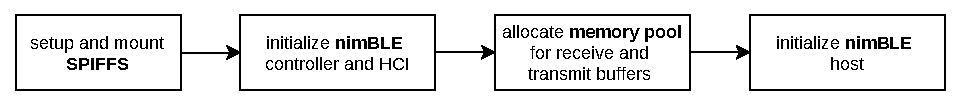
\includegraphics[width=1\textwidth]{graphics/ablauf_anwendung_teil_1.pdf}
    \caption[Ablauf beider Anwendungen (Teil 1)]{Ablauf beider Anwendungen (Teil 1)}
    \label{fig: impl ablauf anwendung teil 1}
\end{figure}
Zu Beginn wird das Dateisystem SPIFFS konfiguriert und initialisiert. Vor dem "`Flashen"' wird eine Partition erstellt, die die jeweiligen Schlüssel und Zertifikate enthält (siehe Sektion \ref{sec: impl prototyp zertifizierungstelle}). Danach wird über \textit{nimBLE} der Bluetooth-Controller im Modus Low Energy und das Host Controller Interface initialisert. Danach wird Speicher für zwei Memory Pools reserviert: einen Memory Pool für empfangene Anwendungsdaten und einen für zu sendende Anwendungsdaten. Schließlich wird der nimBLE-Host in einem neuen Task initialisiert, um das Event Handling für L2CAP und GAP separiert von der Anwendung zu betreiben.
\\\\
Die Abb. \ref{fig: impl ablauf anwendung server teil 2} zeigt den weiteren Ablauf der Server-Anwendung.
\begin{figure}[H]
    \centering
    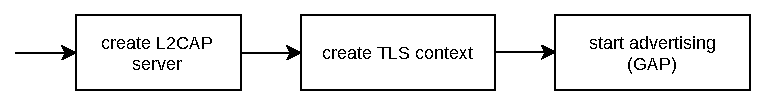
\includegraphics[width=0.8\textwidth]{graphics/ablauf_anwendung_teil_2_server.pdf}
    \caption[Ablauf der Server-Anwendung (Teil 2)]{Ablauf der Server-Anwendung (Teil 2)}
    \label{fig: impl ablauf anwendung server teil 2}
\end{figure}
Zunächst wird der L2CAP-Server erstellt. Somit wird das L2CAP Event Handling aktiv. Anschließend wird der TLS-Kontext erstellt. Er benötigt den privaten Schlüssel und das Zertifikat des Fahrzeugs sowie das Root-Zertifikat. Zudem verlangt er nach den Funktionen für das Senden bzw. Empfangen von Daten durch den Transport (L2CAP). Danach beginnt die Server-Anwendung mit dem Advertising mithilfe von GAP. Dabei werden Connectable Undirected Advertising Events als Broadcast gesendet, in denen die öffentliche Bluetooth-Adresse des Server-Mikrocontrollers angegeben wird. Nun ist auch das GAP Event Handling aktiv.
\\\\
In Abb. \ref{fig: impl ablauf anwendung client teil 2} ist der weitere Ablauf der Client-Anwendung dargestellt.
\begin{figure}[H]
    \centering
    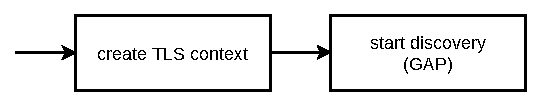
\includegraphics[width=0.6\textwidth]{graphics/ablauf_anwendung_teil_2_client.pdf}
    \caption[Ablauf der Client-Anwendung (Teil 2)]{Ablauf der Client-Anwendung (Teil 2)}
    \label{fig: impl ablauf anwendung client teil 2}
\end{figure}
Die Client-Anwendung erstellt ebenfalls einen TLS-Kontext, nur dass hier der private Schlüssel und das Zertifikat für den Client und nicht für das Fahrzeug benötigt wird. Danach wird mittels GAP nach Advertising Events gescannt (General Discovery Mode). Somit wird das GAP Event Handling aktiv.
\\\\
Mittels der beiden Event Handlings bauen Server und Client erst eine Verbindung über GAP auf und anschließend eine Verbindung über einen neuen L2CAP-Channel. Daraufhin wird der TLS-Handshake ausgeführt. Dabei senden die Anwendungen über L2CAP Service Data Units, deren maximale Länge der Maximum Transmission Unit (MTU) entspricht. Empfängt eine Anwendung eine SDU, speichert sie die SDU im Memory Pool für empfangene Anwendungsdaten (RX-Buffer). Der RX-Buffer ist in Blöcke gleicher Länge aufgeteilt, die jeweils eine MTU speichern können. Jede im RX-Buffer gespeicherte SDU nimmt einen dieser Blöcke ein. Möchte nun die Anwendung eine bestimmte Anzahl an Bytes empfangen, prüft sie zunächst, ob sich eine oder mehrere SDUs im RX-Buffer befinden. Sie liest ggf. die geforderte Byteanzahl aus der SDU und lässt einen Pointer auf das nächst zu lesende Byte zeigen. Für den Fall eines leeren RX-Buffers, wartet die Anwendung (mittels Semaphores) bis eine SDU empfangen und in den RX-Buffer geschrieben wurde.
\\\\
Schlägt der TLS-Handshake fehl, stoppen beide Anwendungen. Anderenfalls erstellt der Client die Subscription mit einem vorgefertigtem Payload. Hat er den Hashwert des Payloads gebildet und signiert, sendet er die Subscription mithilfe des TLS-Kontextes an den Server. Dieser verifiziert die Subscription (siehe Sektion \ref{sec: impl verbindungsaufbau und autorisierung}). Wurde die Subscription erfolgreich verifiziert, erfolgt die Bestätigung auf der Konsole. Anderenfalls stoppt die jeweilige Anwendung.